
\begin{table}[!htb] 
	\centering
	\begin{tabular}{c|cccccccc}
	\hline \hline 
  		Process   & Signal(125)	& Signal(150)	& qqWW 	& ggWW 	& VV  	& Top 	& Wjets	& Wgamma \\
	\hline 
	  	Yields    & 36.4 		& 165.6			& 696.2	& 47.2 	& 16.3 	& 119.4	&84.9	& 13.6 \\ 
	\hline \hline 
	\end{tabular}
	\label{tab:exp_sig_understand}
	\caption{Signal and Background yields in 5 \ifb.} 
\end{table} 

\begin{figure}[!hbtp]
	
	%
	\centering
	\subfigure[Data]{
	\centering
	\label{subfig:template_data_125}
		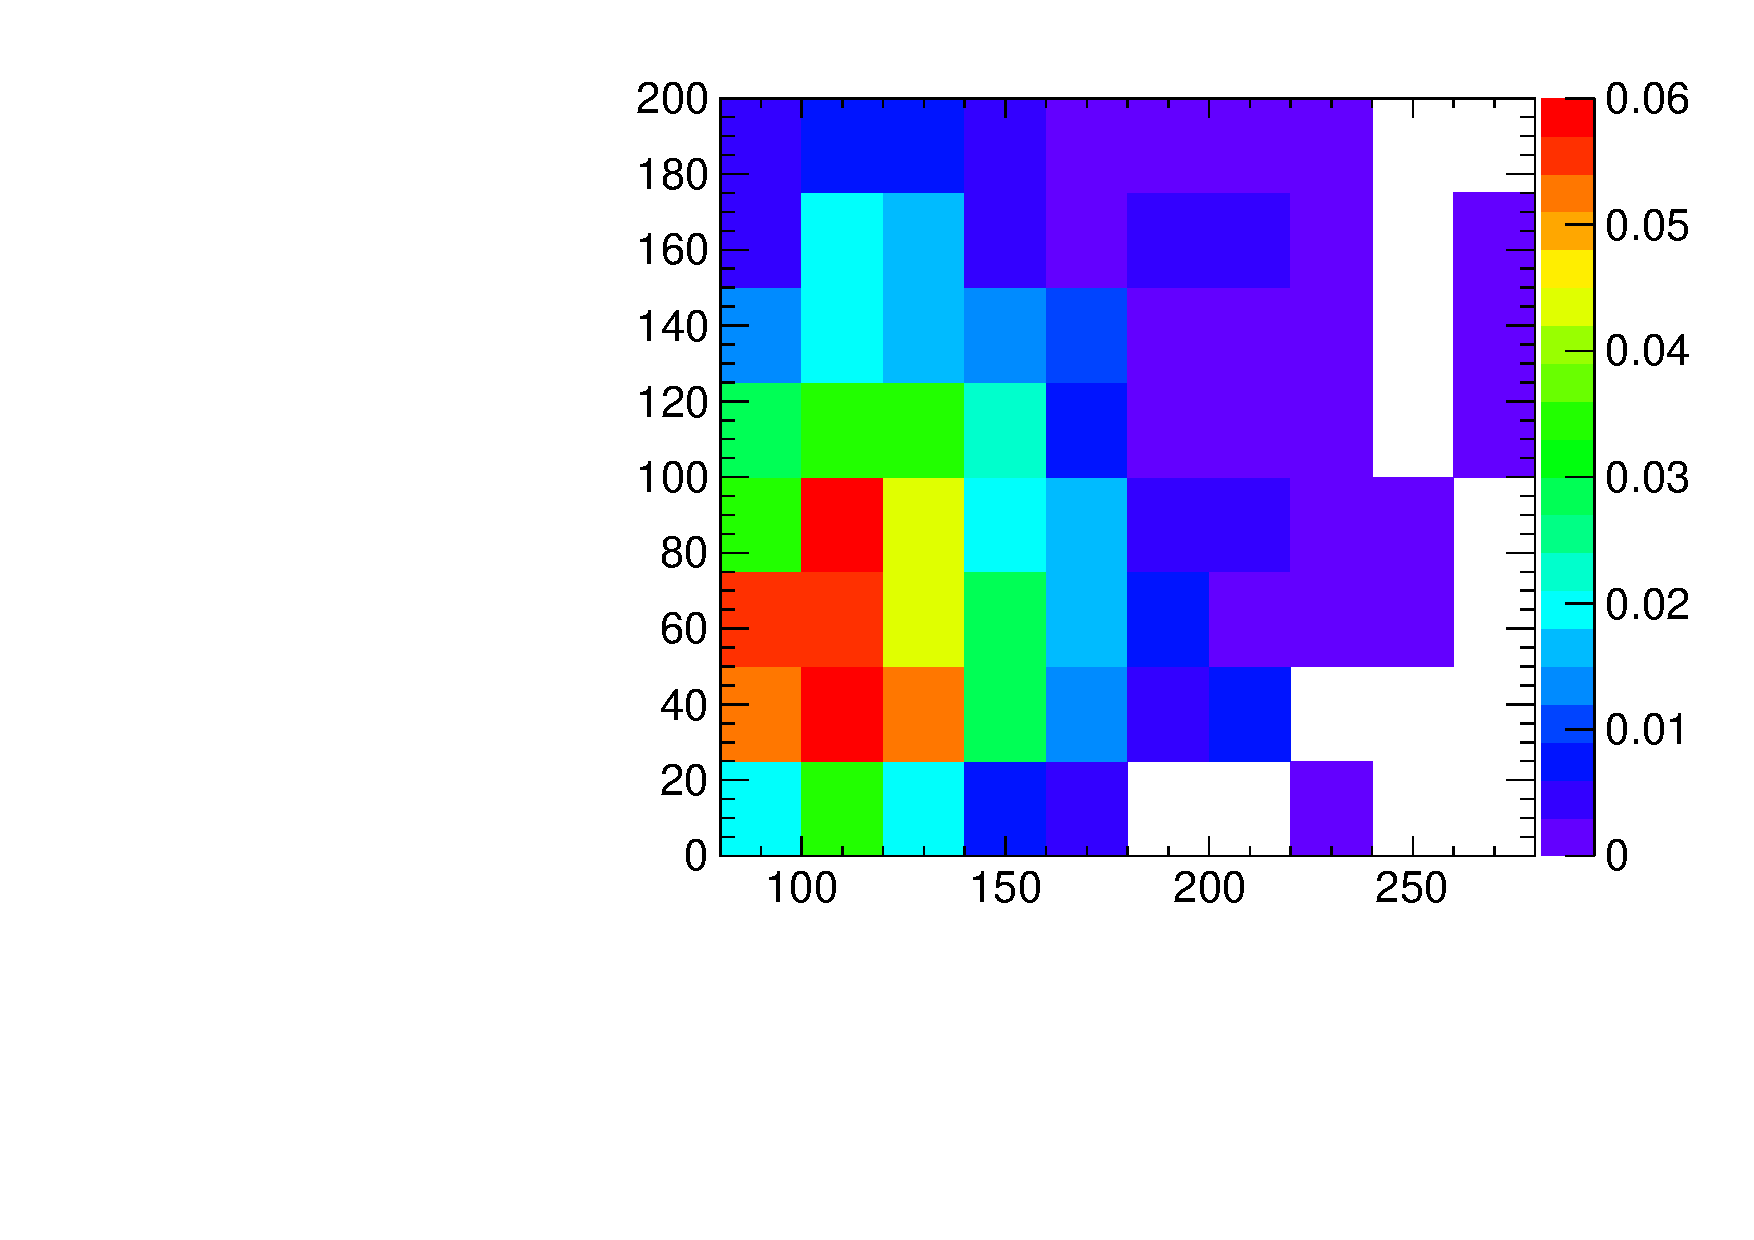
\includegraphics[width=.40\textwidth]{figures/templates/data_2D_mH125_0j_of.pdf}
	}
	
	%
	\centering
	\subfigure[Signal \mHi=125 \GeV]{
	\centering
	\label{subfig:template_sig_125}
		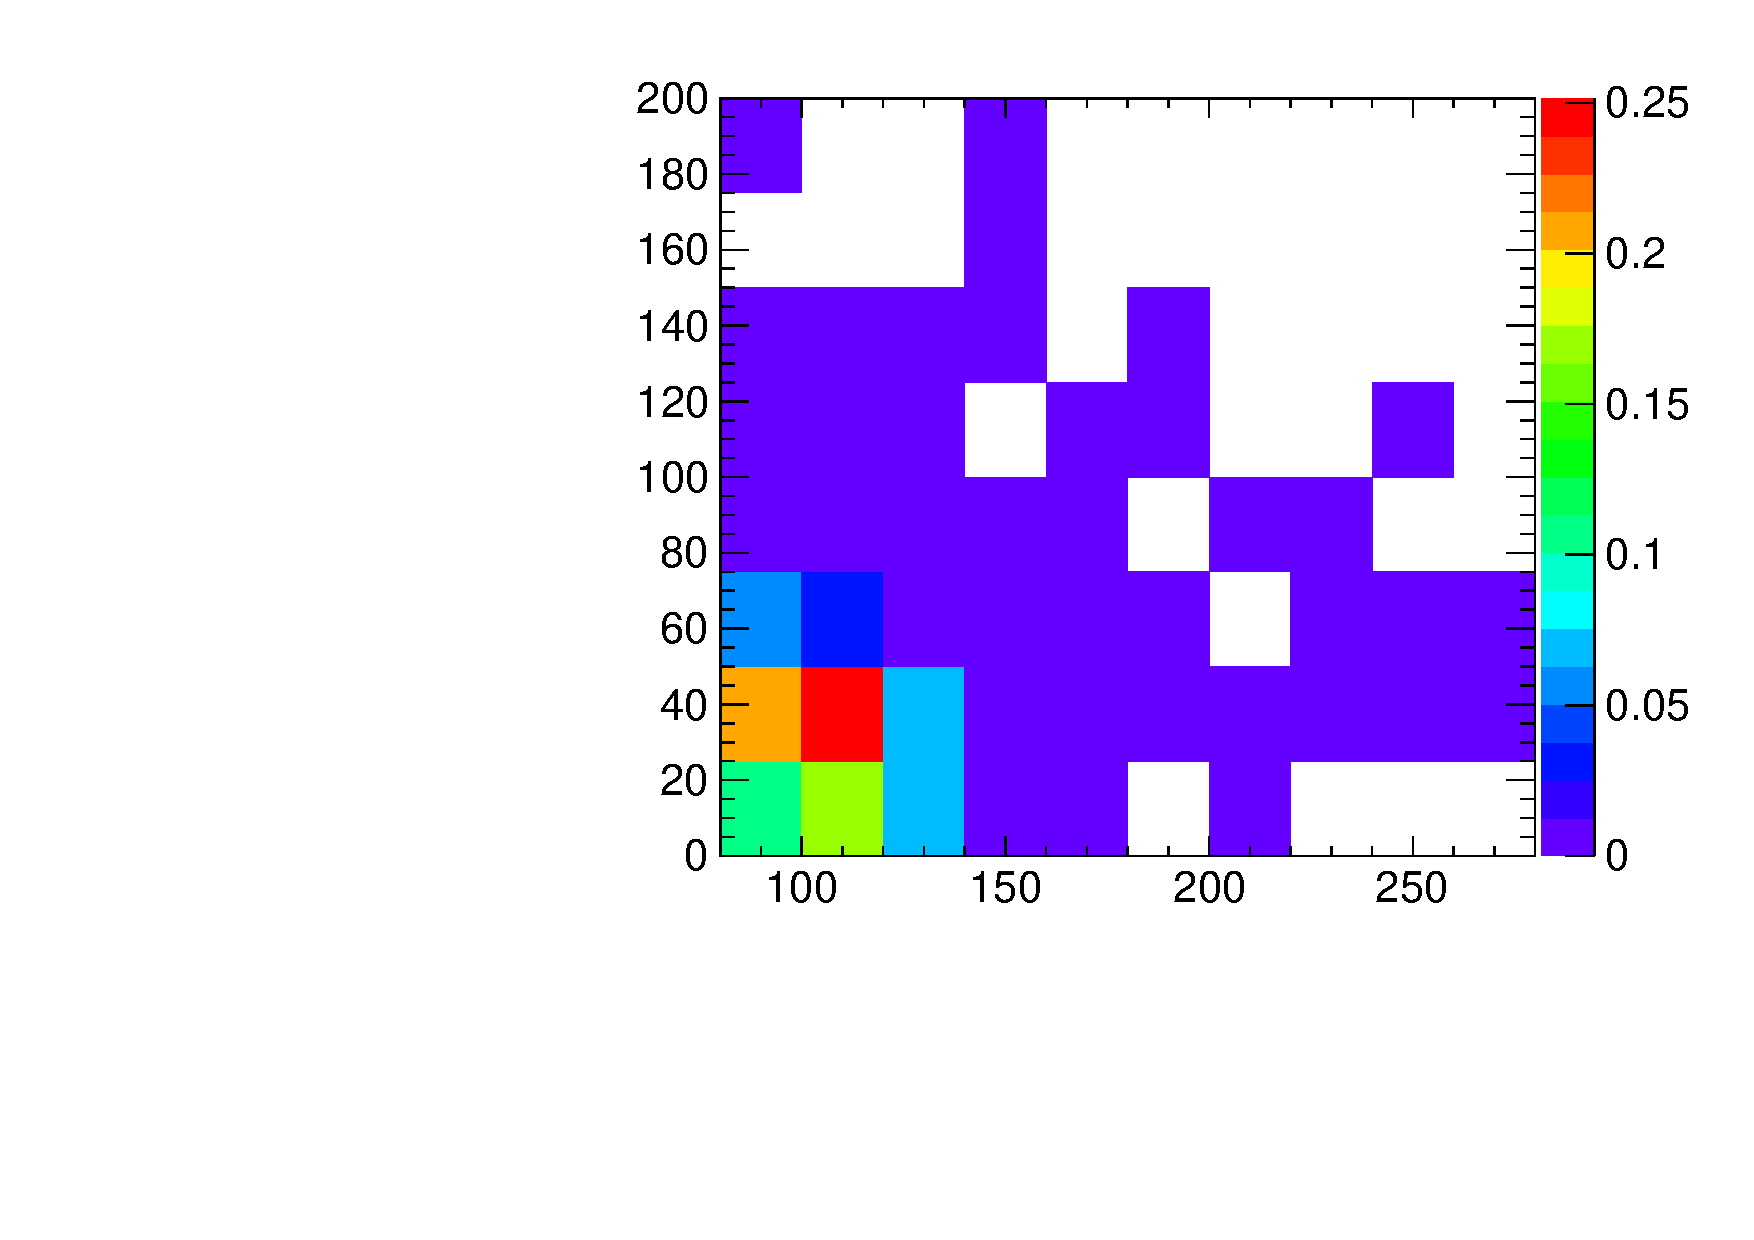
\includegraphics[width=.30\textwidth]{figures/templates/sig_2D_mH125_0j_of.pdf}
	}
	\subfigure[Signal \mHi=150 \GeV]{
	\centering
	\label{subfig:template_sig_150}
		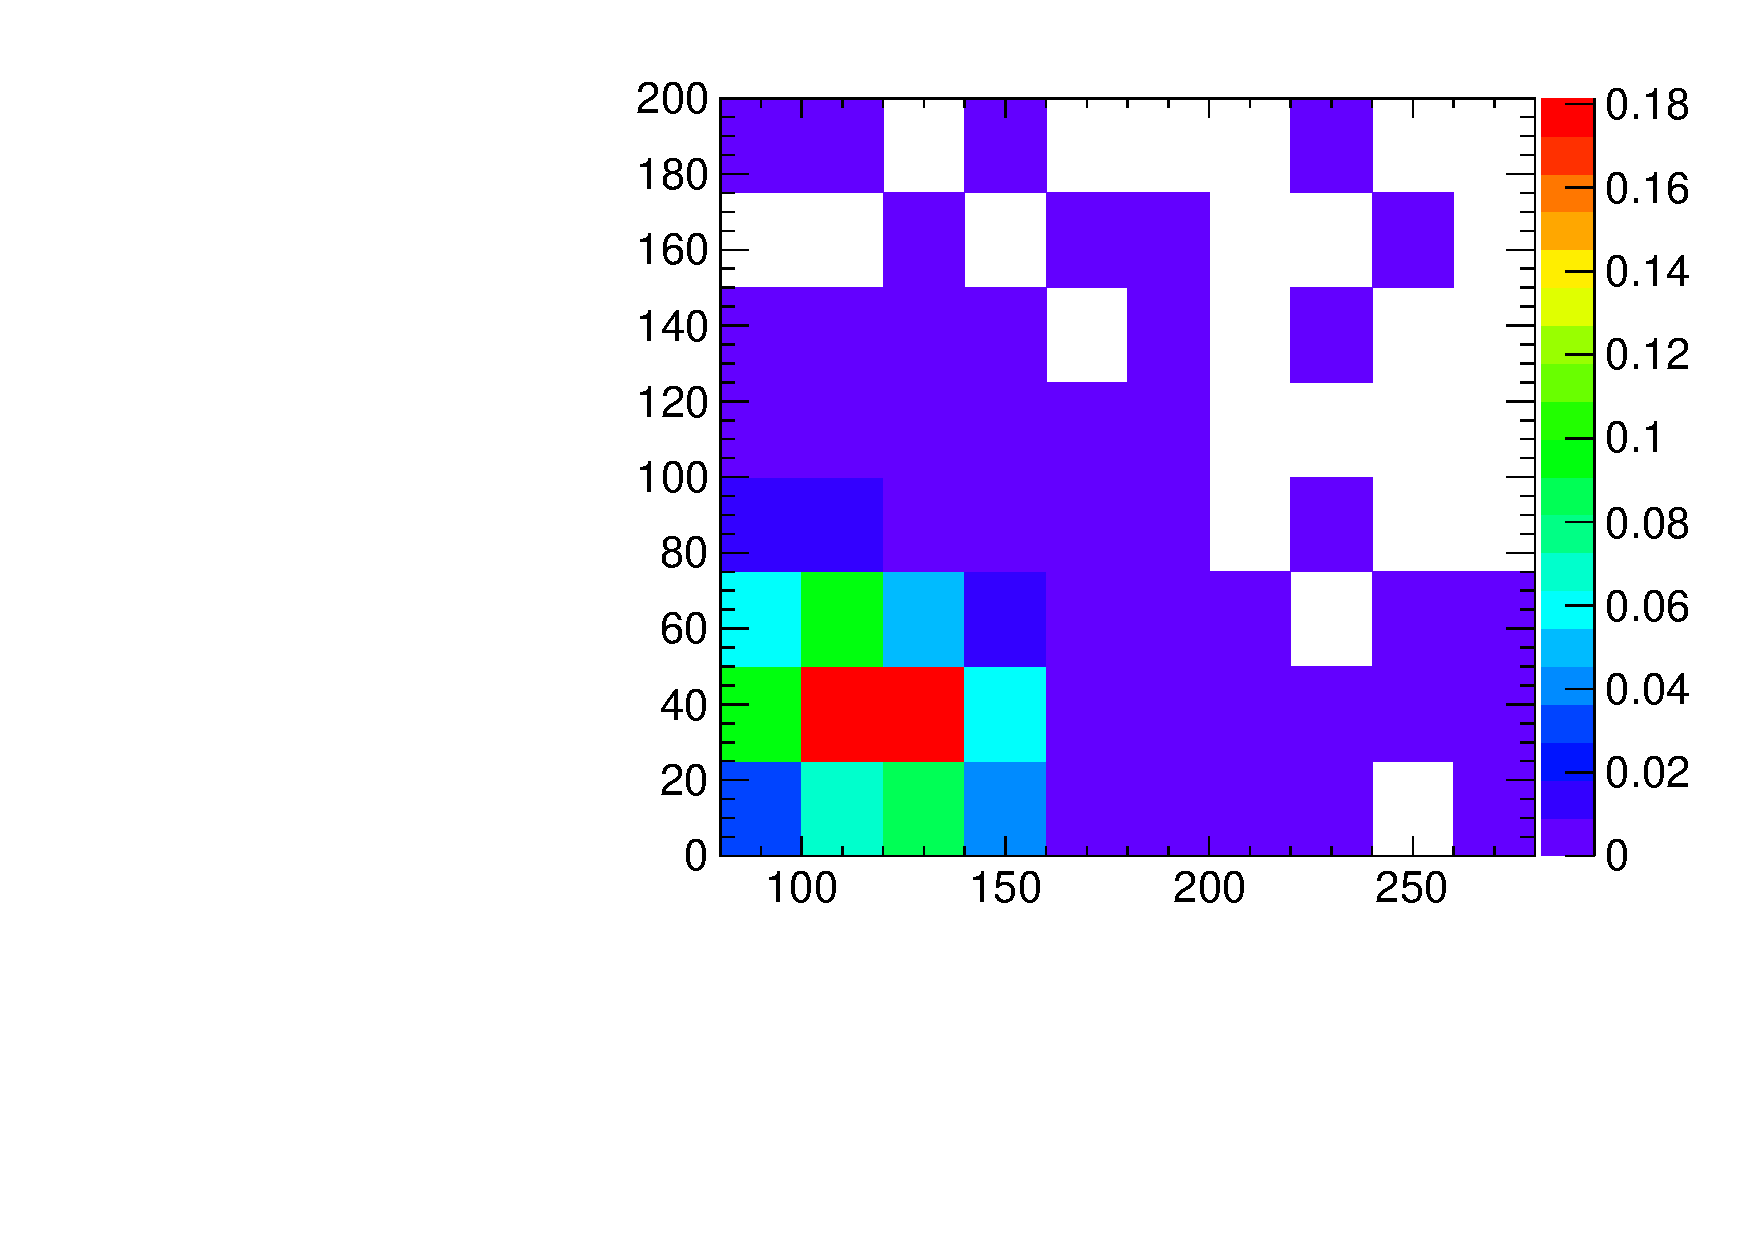
\includegraphics[width=.30\textwidth]{figures/templates/sig_2D_mH150_0j_of.pdf}
	}
	\subfigure[qqWW]{
	\centering
	\label{subfig:template_qqWW_125}
		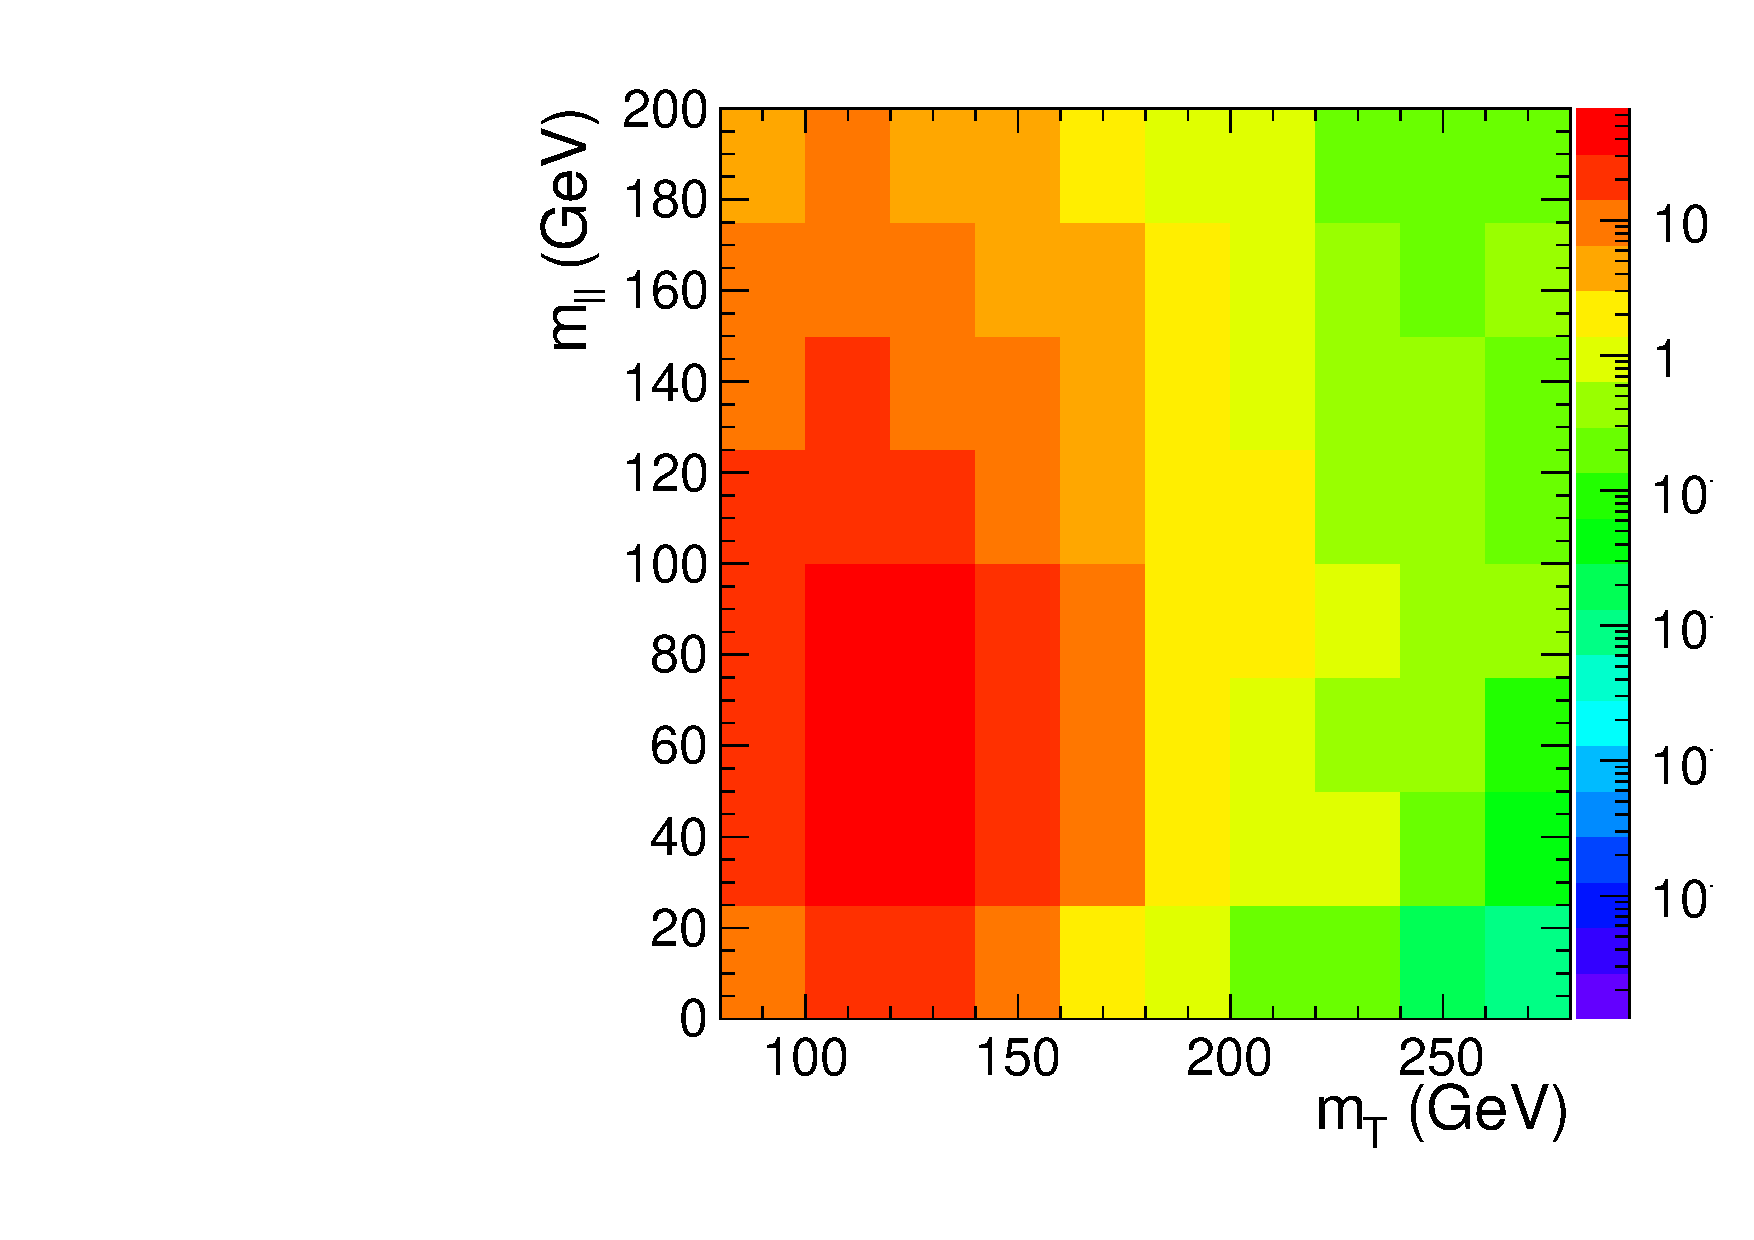
\includegraphics[width=.30\textwidth]{figures/templates/qqWW_2D_mH125_0j_of.pdf}
	}

	%
	\centering
	\subfigure[ggWW]{
	\centering
	\label{subfig:template_ggWW_125}
		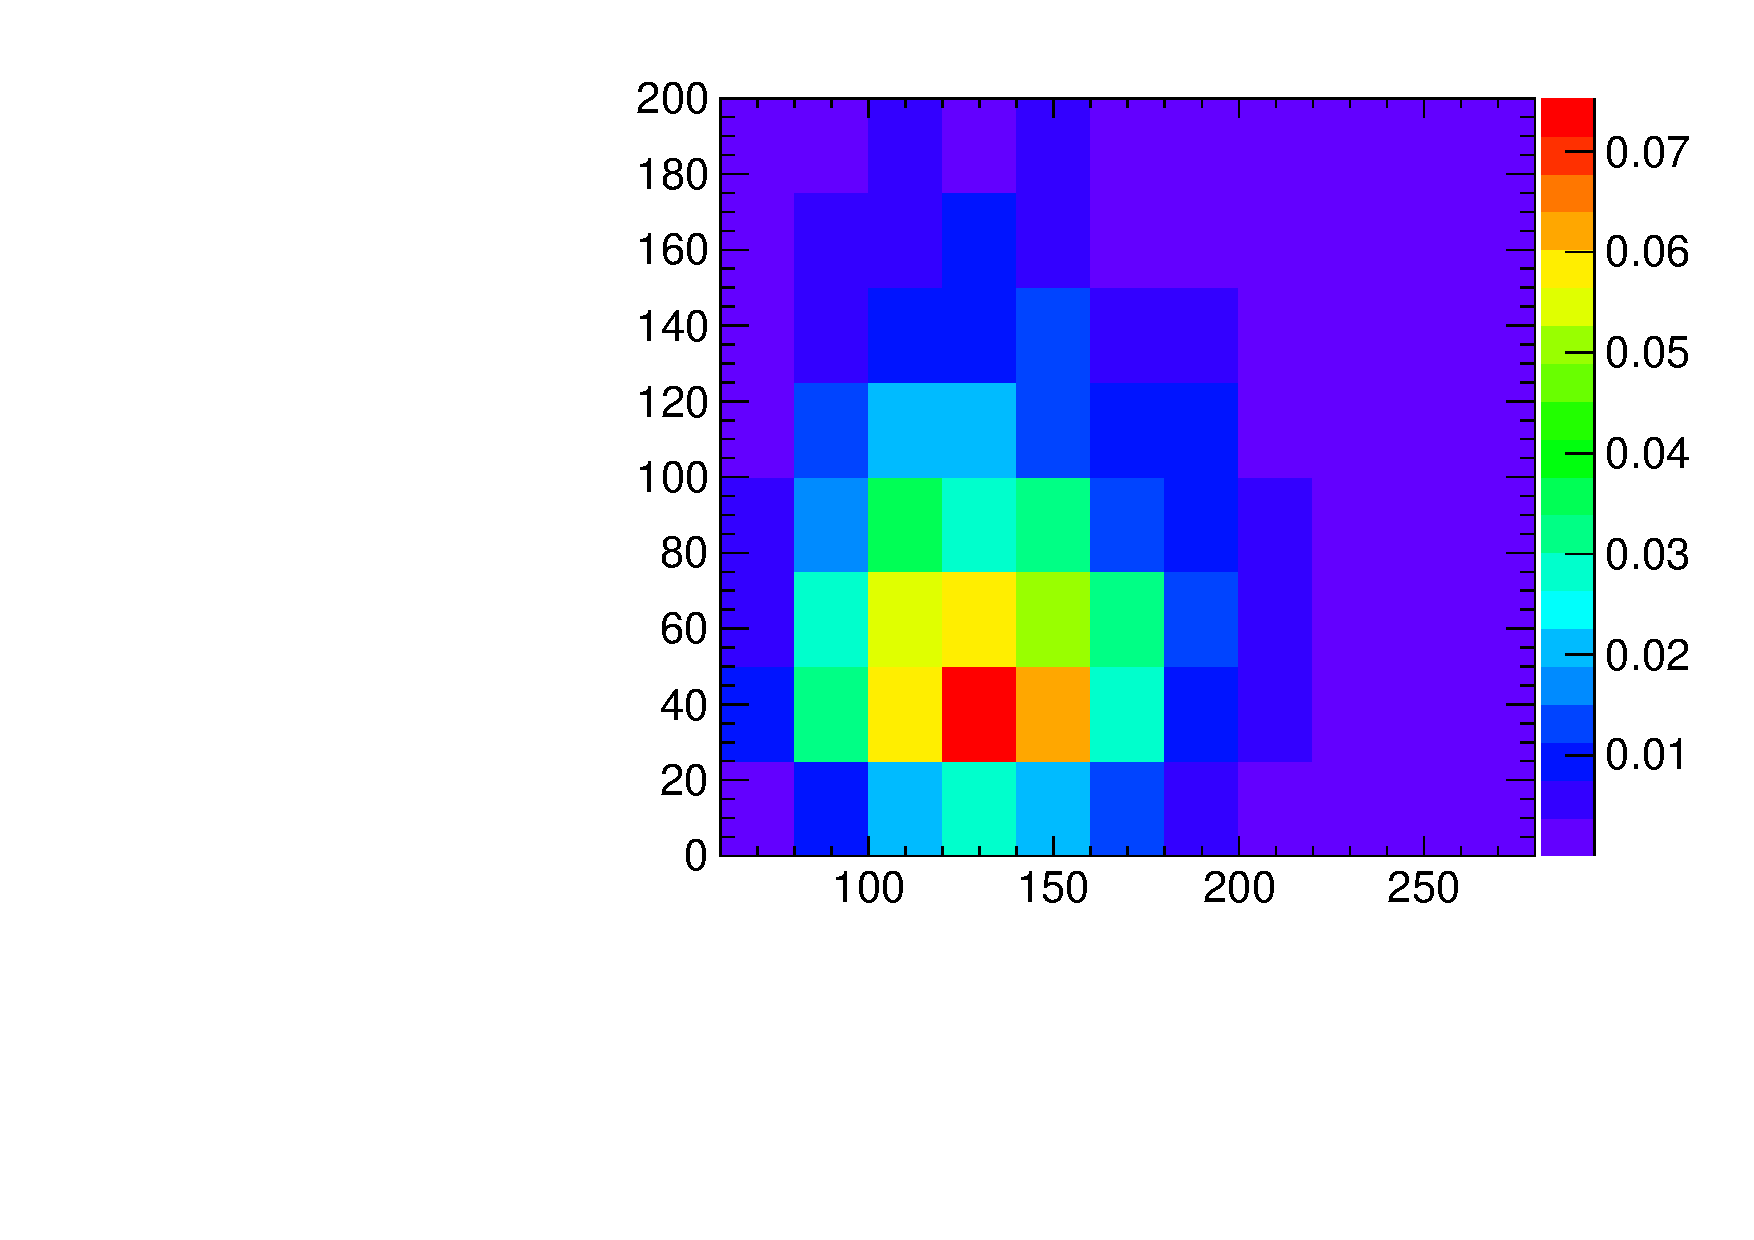
\includegraphics[width=.30\textwidth]{figures/templates/ggWW_2D_mH125_0j_of.pdf}
	}
	\subfigure[Top]{
	\centering
	\label{subfig:template_top_125}
		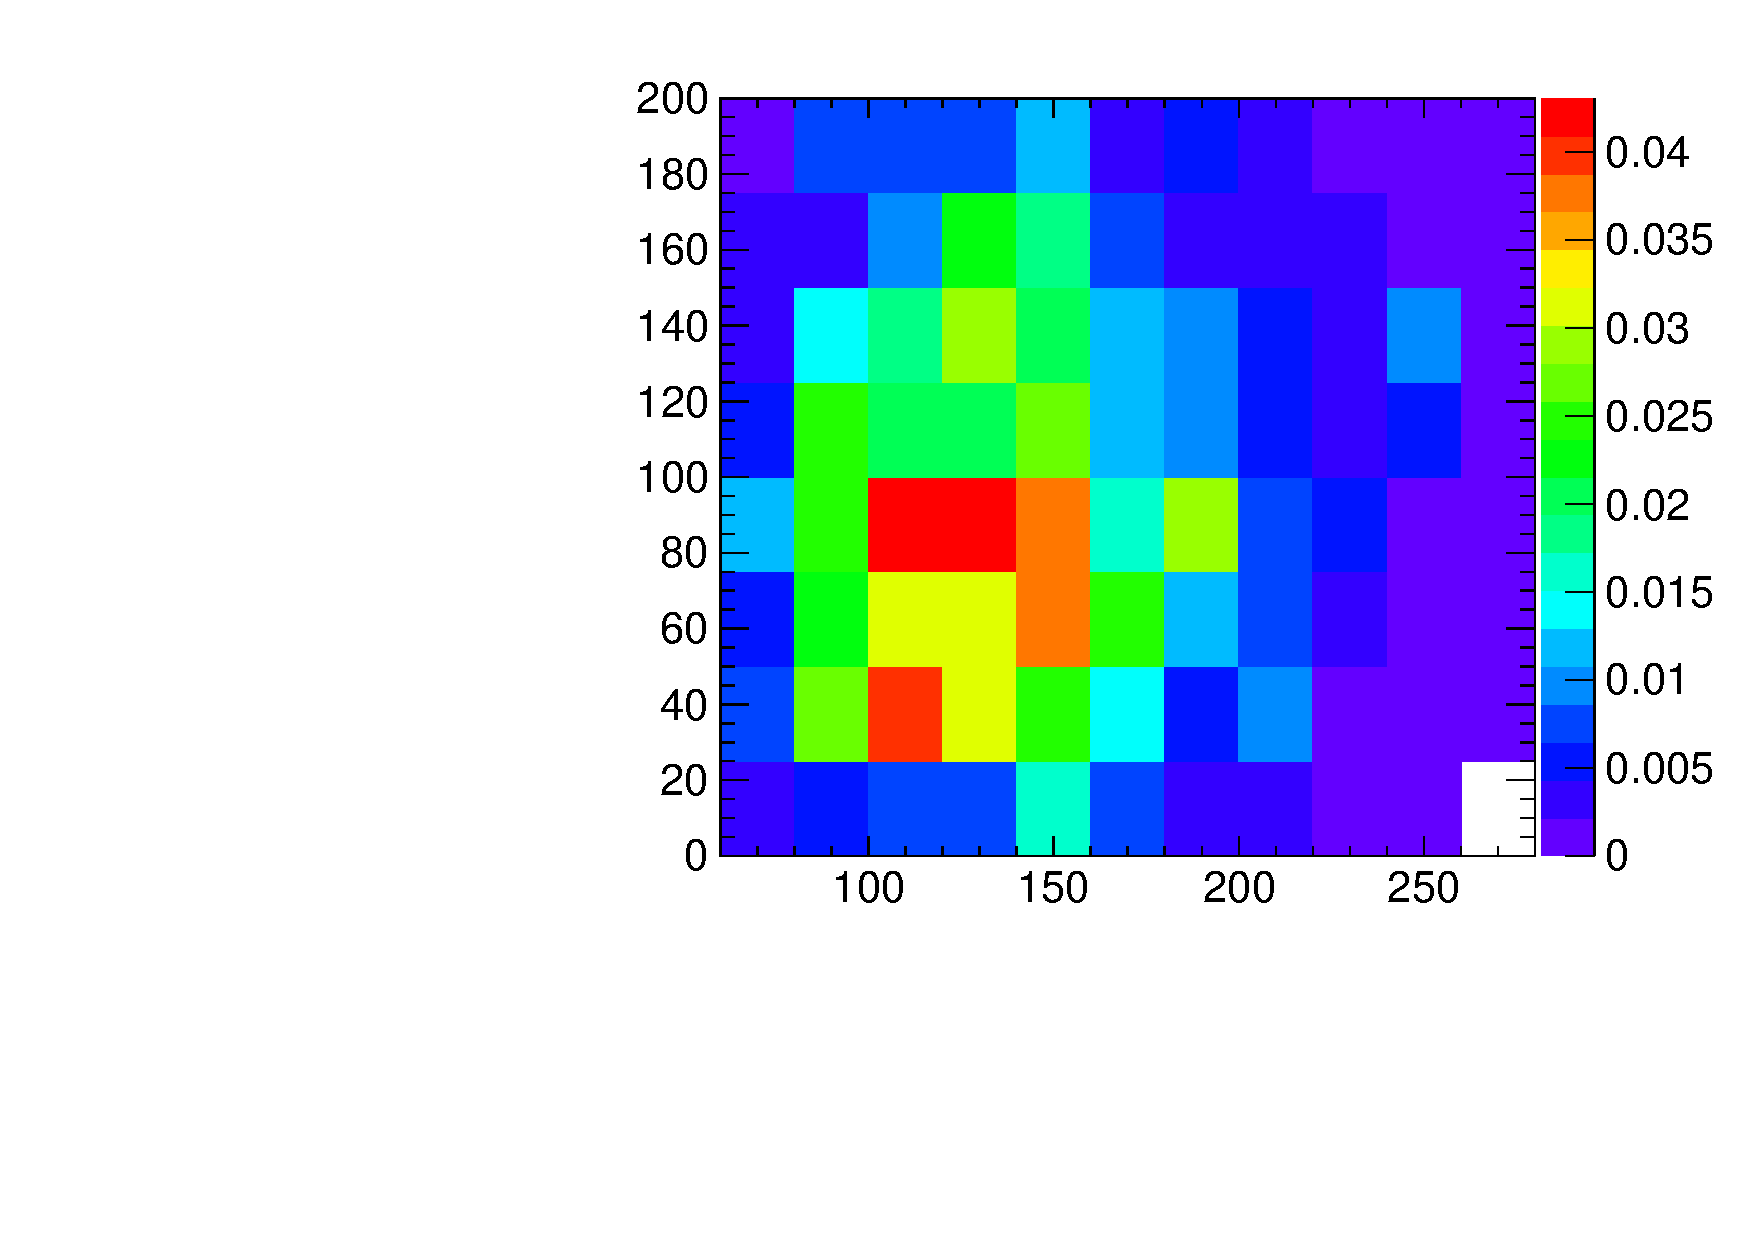
\includegraphics[width=.30\textwidth]{figures/templates/Top_2D_mH125_0j_of.pdf}
	}
	\subfigure[Wjets]{
	\centering
	\label{subfig:template_Wjets_125}
		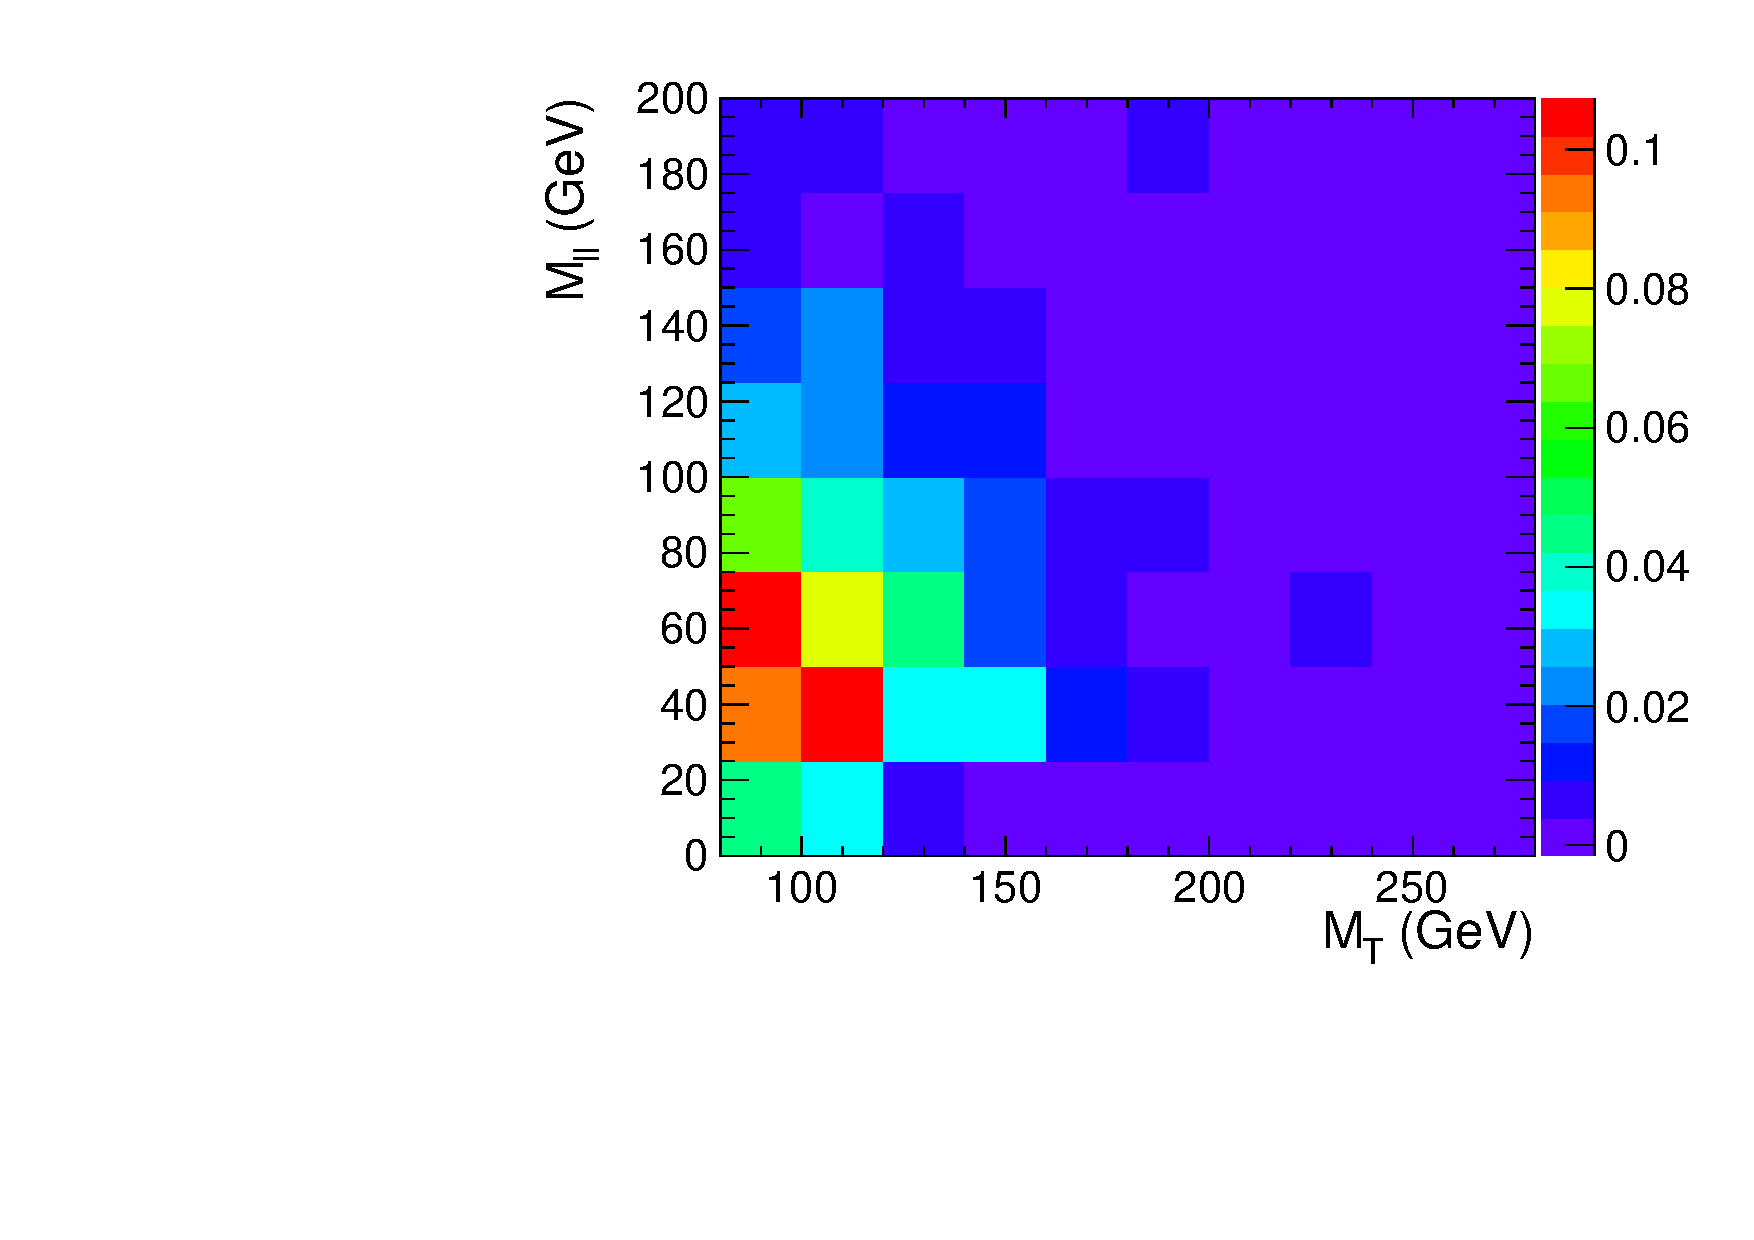
\includegraphics[width=.30\textwidth]{figures/templates/Wjets_2D_mH125_0j_of.pdf}
	}
	
	%
	\centering
	\subfigure[VV]{
	\centering
	\label{subfig:template_VV_125}
		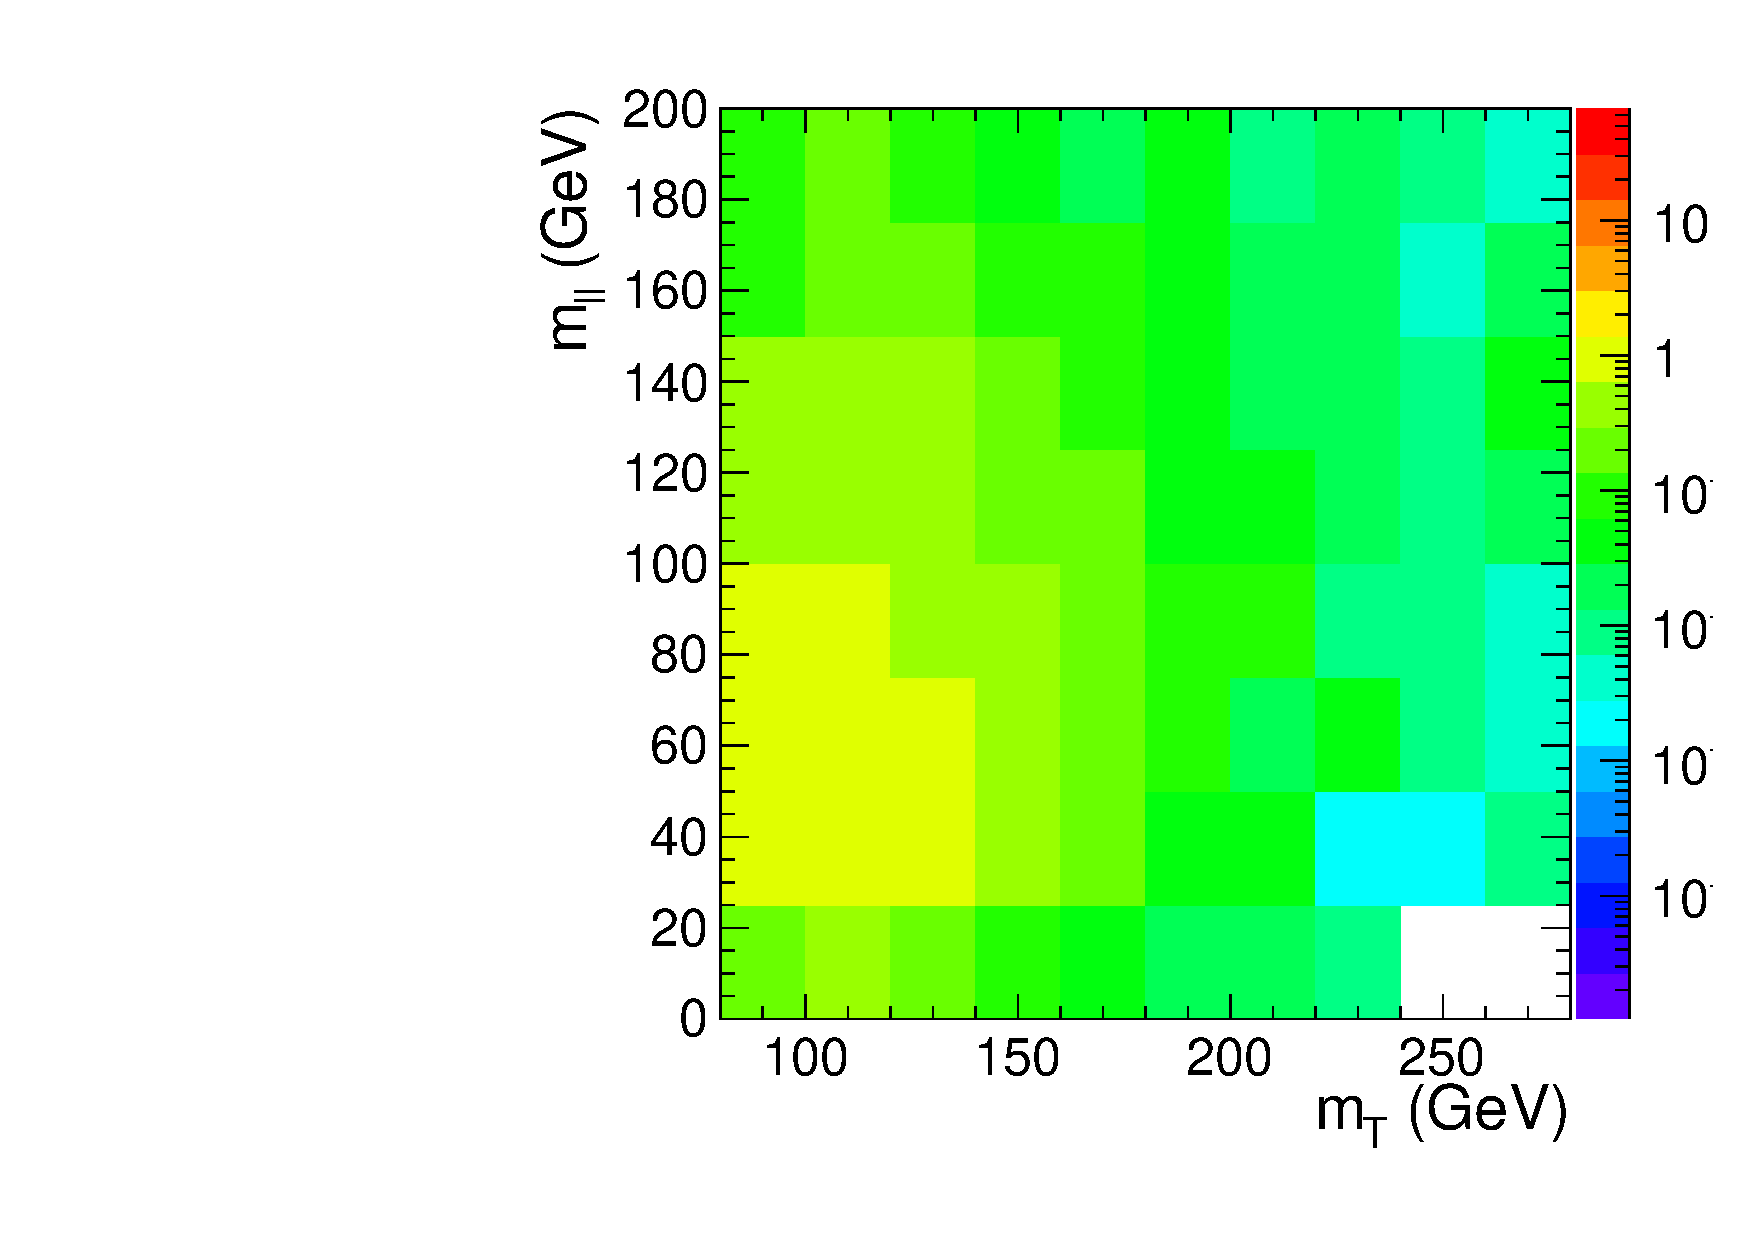
\includegraphics[width=.30\textwidth]{figures/templates/VV_2D_mH125_0j_of.pdf}
	}
	\centering
	\subfigure[Wgamma]{
	\centering
	\label{subfig:template_Wgamma_125}
		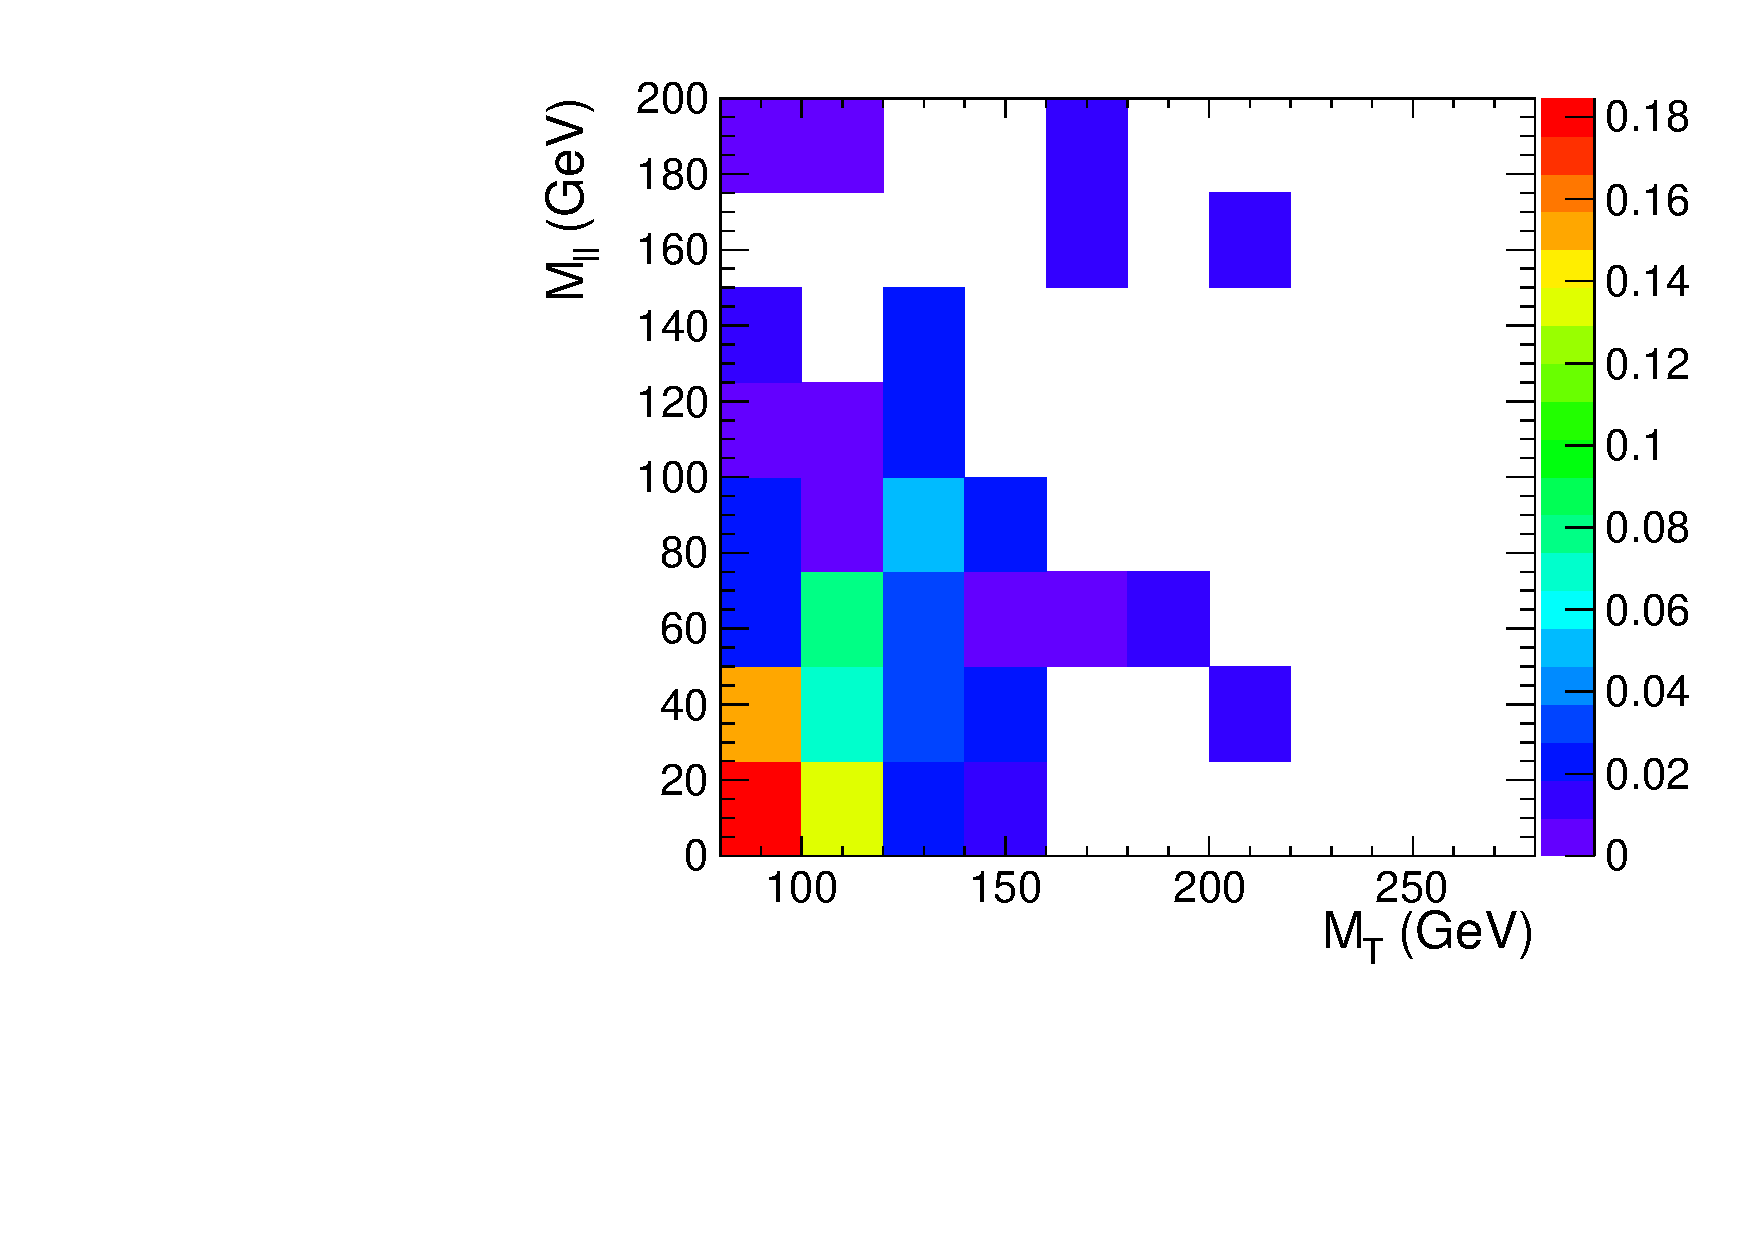
\includegraphics[width=.30\textwidth]{figures/templates/Wgamma_2D_mH125_0j_of.pdf}
	}



	\caption{2D templates for data, signal, and backgrounds in 5 \ifb. 
			Templates are normalized to unit area.} 
	\label{fig:templates_eyefit}

\end{figure}





